We apply a data-driven method to estimate the $\dyll$ contributions in the 
same flavor $\ell^+\ell^-$ final states. This method also provides an estimate 
for the \emph{peaking component} of $WZ$ and $ZZ$ contributions, in which both 
leptons come from the same $Z$ boson.

The expected contributions from $\dyll$ events outside the $Z$-mass 
region in data can be estimated by counting the number of events near 
the $Z$ mass region in data, subtracting from it the non-$Z$ contributions, 
and scaling it by a ratio $R_{out/in}$ defined as
%%%%%%%%%%%%%%%%%%%%%%%%%%%%%%
\begin{eqnarray}
N_{out}^{ll,exp} = R_{out/in}^{ll,loose}(N_{in}^{ll} - 0.5N_{in}^{e\mu}k_{ll}), 
\label{eq:dyest}
\end{eqnarray}
%%%%%%%%%%%%%%%%%%%%%%%%%%%%%%
where $k_{ee} = \sqrt{\frac{N_{in}^{ee,loose}}{N_{in}^{\mu\mu,loose}}}$ for 
$\dyee$ and $k_{mm} = \sqrt{\frac{N_{in}^{\mu\mu,loose}}{N_{in}^{ee,loose}}}$ 
for $\dymm$. $R_{out/in}$ is obtained from simulation as 
$N_{out}^{MC}/N_{in}^{MC}$ with no $\met$ cut (referred to as a loose 
selection). The non-$Z$ contributions close to the $Z$-mass region in data is 
estimated from the number of events in the $e^\pm\mu^\mp$ final state 
$N_{in}^{e\mu}$, applying a correction factor that normalizes the 
electron-to-muon efficiency $k_{ee/\mu\mu}$. 
%To validate this method, we apply it first on events with no $\met$ cut. 
%These events are dominated by $\dyll$. A good agreement within 10\% between 
%the predictions from the data-driven method and simulation is observed. 
The method relies on on the assumption that the dependence of the ratio $R_{out/in}$ 
on the $\met$ cut is well modelled by the simulation and is relatively flat. 
An estimate of the degree to which this assumption fails is shown in  
Figure~\ref{fig:routin_met}, and gives the estimate of the systematic uncertainty
of this background prediction. The ratio $R_{out/in}$ is observed to be
different for the dielectron and dimuon final states, as expected due to 
the different $p_{T}$ cuts on the electron and muon candidates.


%%%%%%%%%%%%%%%%%%%%%%%%%%%%%%
\begin{figure}[!htbp]
\begin{center}
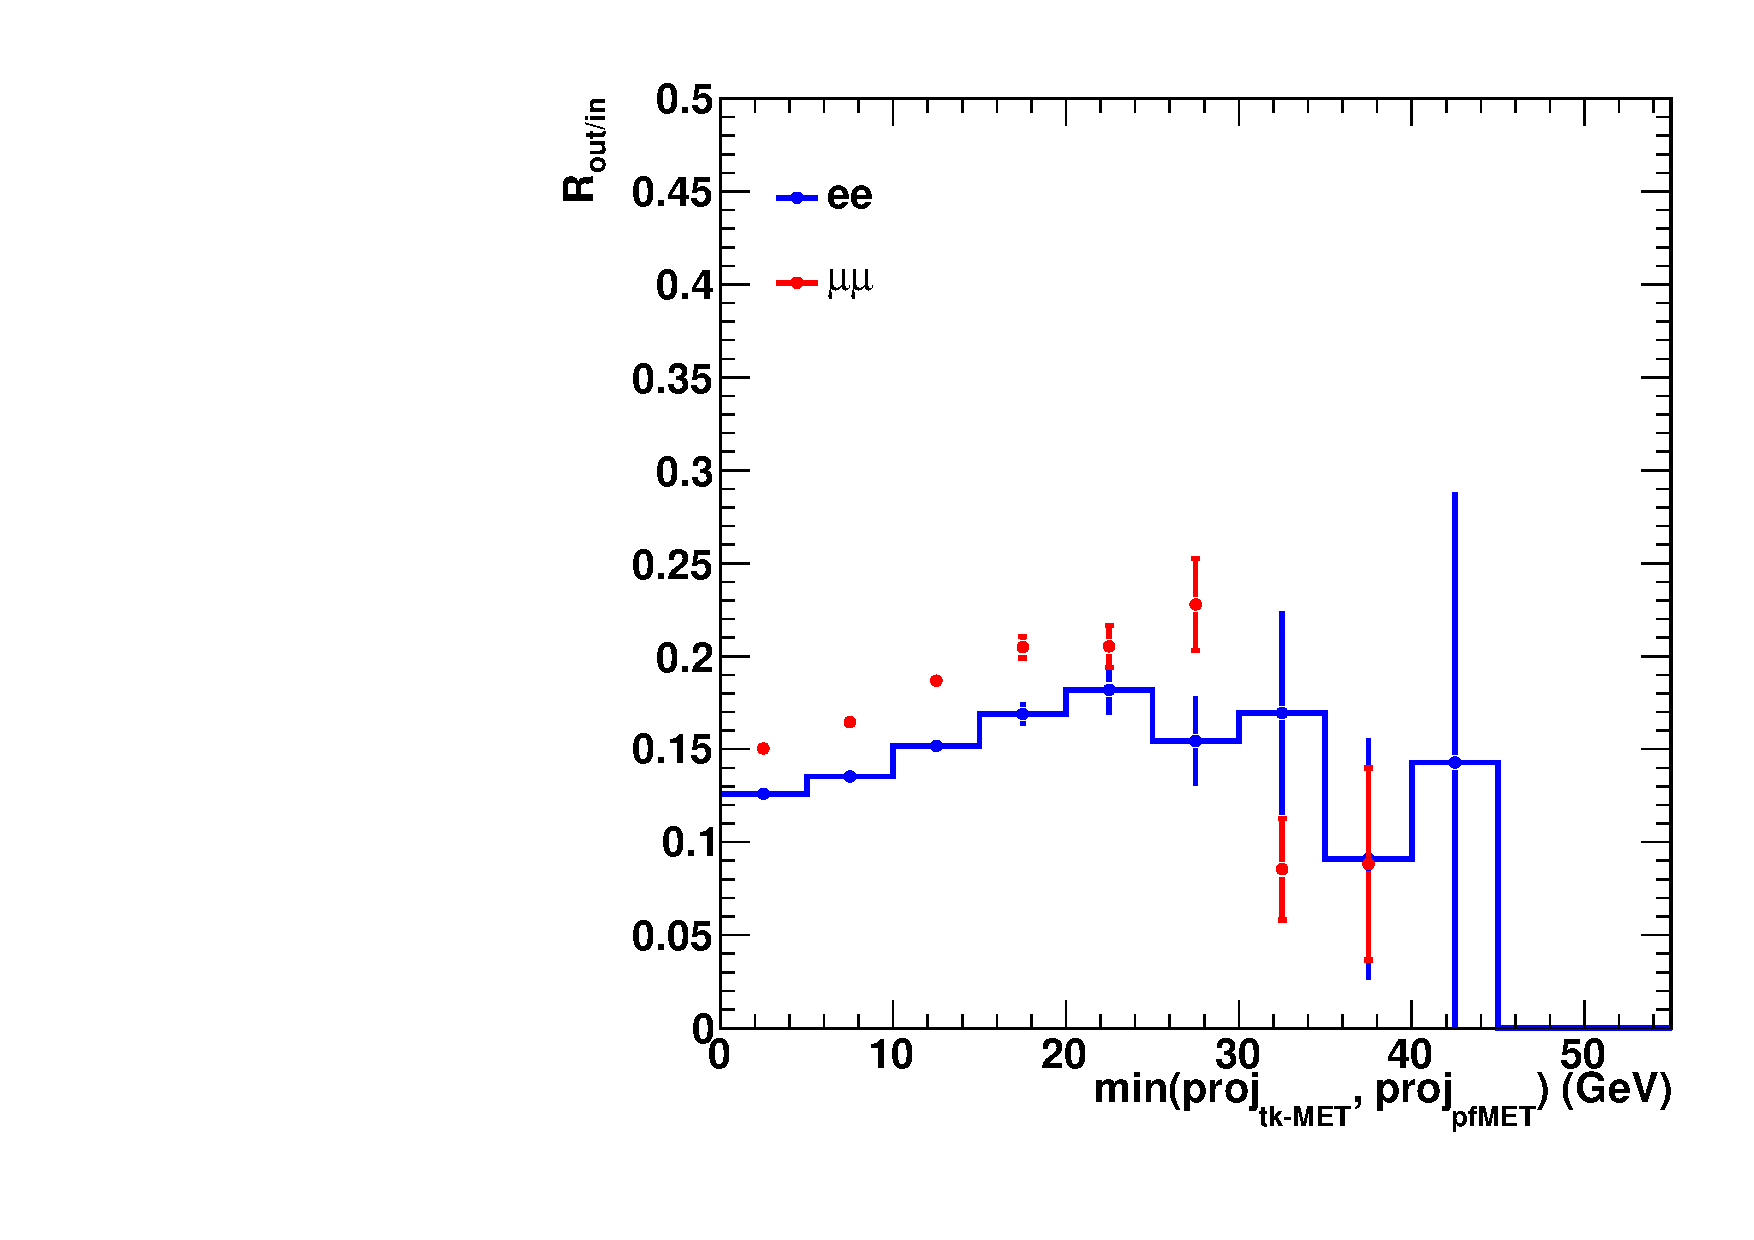
\includegraphics[width=0.3\textwidth]{figures/Routin_mc_0Jet.pdf}
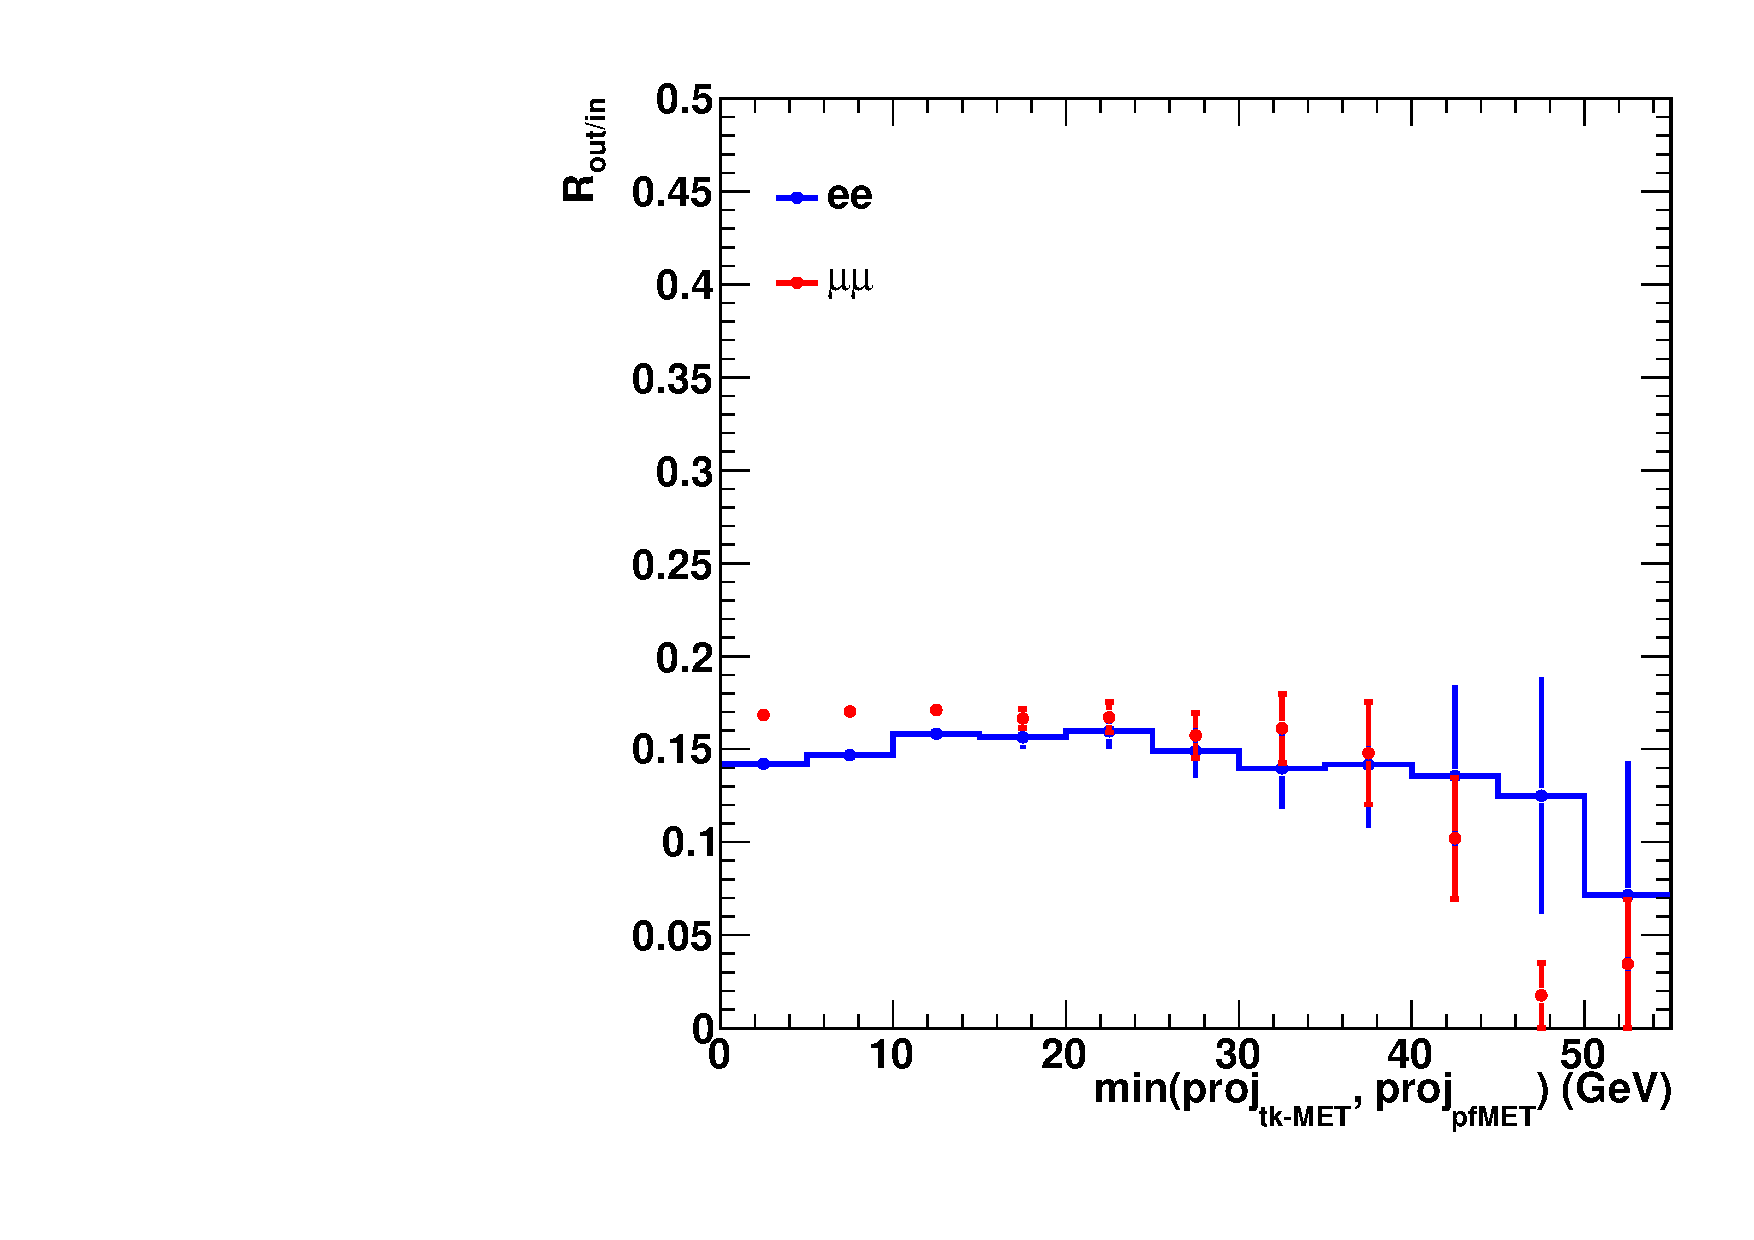
\includegraphics[width=0.3\textwidth]{figures/Routin_mc_1Jet.pdf}
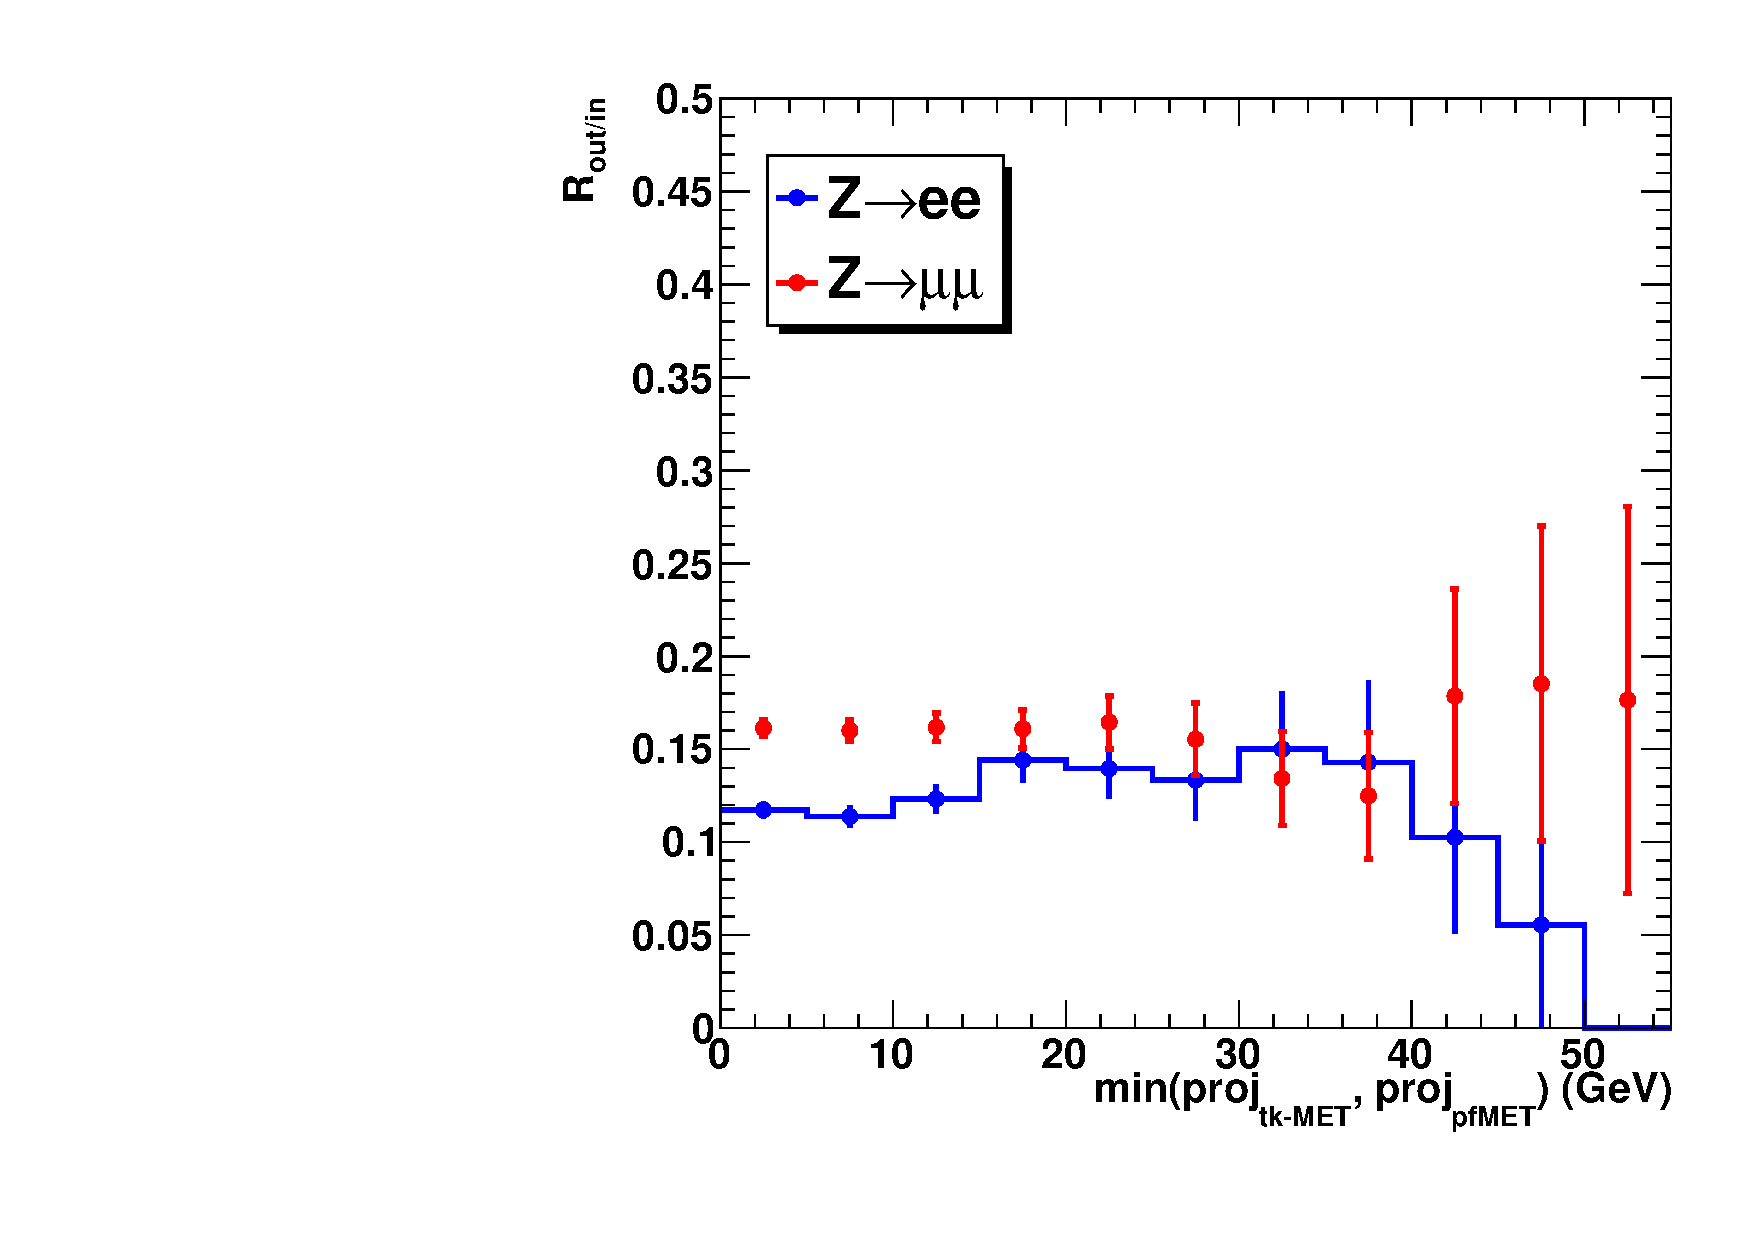
\includegraphics[width=0.3\textwidth]{figures/Routin_mc_2Jet.pdf}
\caption{ The ratio $R_{out/in}$ as a function of the $\met$ cut obtained using MC in the 
0-Jet (left), 1-Jet (middle) and 2-Jet (right) bins. }
\label{fig:routin_met}
\end{center}
\end{figure}
%%%%%%%%%%%%%%%%%%%%%%%%%%%%%%
